
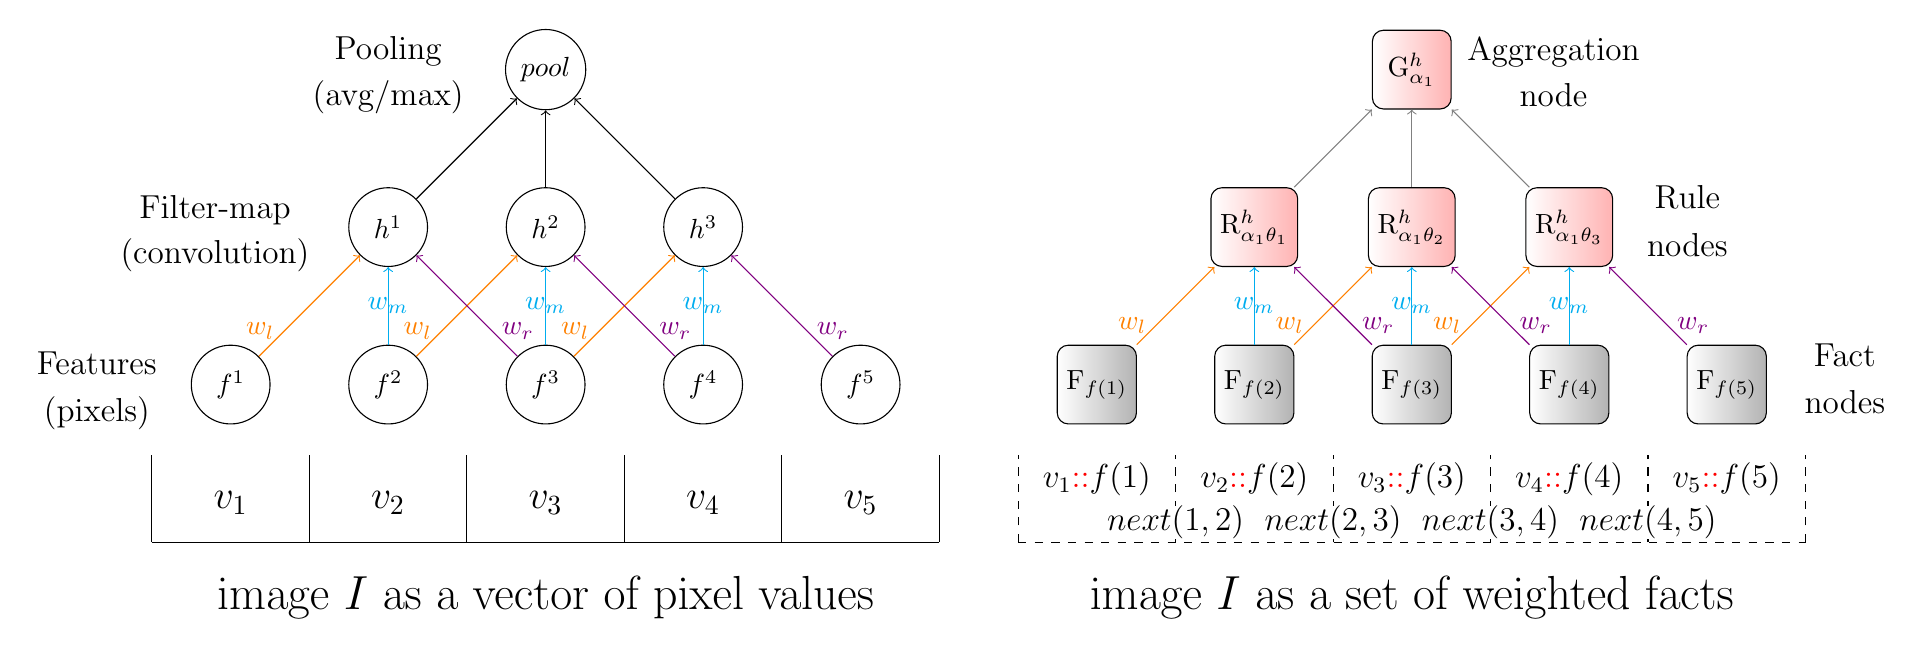
\begin{tikzpicture}
[transform shape,rotate=0, node distance=2.0cm and 2.0cm,
ar/.style={->,>=latex},
mynode/.style={
  draw, scale = 1.0,  minimum size=1cm, rounded corners,left color=white,
  minimum height=1cm,
  align=center
  }
]

\tikzstyle{neuron}  =  [circle, draw, scale = 1.0,  minimum size=1cm]
\tikzstyle{grbond}  =  [mynode, right color=red!30!white]
\tikzstyle{gratom}  =  [mynode]
\tikzstyle{grgroup} =  [mynode, right color=brown!30!white]
\tikzstyle{grexpl}  =  [mynode, right color=red!30!white]
\tikzstyle{edgenode}  =  [thin, draw=black, align=center,fill=white,font=\small]

%------1
\begin{scope}[xshift=0cm,yshift=0cm]

\begin{scope}[xshift=-1cm, yshift=-2cm]

\draw[step=2.0,black,thin] (0,0) grid (10,1.1);

\node at (1,0.5) {\Large $v_1$};
\node at (3,0.5) {\Large $v_2$};
\node at (5,0.5) {\Large $v_3$};
\node at (7,0.5) {\Large $v_4$};
\node at (9,0.5) {\Large $v_5$};


\node[] (gh2) [xshift=5cm, yshift=-0.7cm] {\LARGE image $I$ as a vector of pixel values};

\end{scope}

\begin{scope}[xshift=0cm]

\node[neuron,label={[xshift=-1.7cm, yshift=-0.5cm]{\large Features}},label={[xshift=-1.7cm, yshift=-1.2cm]{\large (pixels)}}] (gh1) {$f^1$};
\node[neuron] (gh2) [right of=gh1] {$f^2$};
\node[neuron] (gh3) [right of=gh2] {$f^3$};
\node[neuron] (gh4) [right of=gh3] {$f^4$};
\node[neuron] (gh5) [right of=gh4] {$f^5$};

\end{scope}

%filters
\begin{scope}[xshift=1cm, yshift=2cm]

\node[neuron,label={[xshift=-2.2cm, yshift=-0.6cm]{\large Filter-map}},label={[xshift=-2.2cm, yshift=-1.2cm]{\large (convolution)}}] (gr1h2) [above of=gh2] {$h^1$};
\node[neuron] (gr1h3) [right of=gr1h2] {$h^2$};
\node[neuron] (gr1h4) [right of=gr1h3] {$h^3$};

\end{scope}

%aggregation
\begin{scope}[xshift = 1cm, yshift=4cm]
\node[neuron, label={[xshift=-2.0cm, yshift=-0.6cm]{\large Pooling}},label={[xshift=-2.0cm, yshift=-1.2cm]{\large (avg/max)}}] (explosive1)  [above of=gr1h3] {$pool$};
\end{scope}


\end{scope}

%---edges1

\draw[orange,->] (gh1) -> node[orange,near start,left] {$w_l$} (gr1h2);
\draw[orange,->] (gh2) -> node[orange,near start,left] {$w_l$} (gr1h3);
\draw[orange,->] (gh3) -> node[orange,near start,left] {$w_l$} (gr1h4);

\draw[cyan,->] (gh2) -> node[cyan] {$w_m$} (gr1h2);
\draw[cyan,->] (gh3) -> node[cyan] {$w_m$} (gr1h3);
\draw[cyan,->] (gh4) -> node[cyan] {$w_m$} (gr1h4);

\draw[violet,->] (gh3) -> node[violet,near start,right] {$w_r$} (gr1h2);
\draw[violet,->] (gh4) -> node[violet,near start,right] {$w_r$} (gr1h3);
\draw[violet,->] (gh5) -> node[violet,near start,right] {$w_r$} (gr1h4);

\draw[->] (gr1h2) -> node[left] {} (explosive1);
\draw[->] (gr1h3) -> node[right] {} (explosive1);
\draw[->] (gr1h4) -> node[right] {} (explosive1);

%---------------2
% % % %maly grounding
\begin{scope}[xshift=11cm,yshift=0cm]

\begin{scope}[xshift=-1cm, yshift=-2cm]

\draw[step=2.0,black,thin,dashed] (0,0) grid (10,1.1);

\node at (1,0.8) {\large  $\scalar{v_1}\textcolor{red}{::} f(1)$};
\node at (3,0.8) {\large  $\scalar{v_2}\textcolor{red}{::} f(2)$};
\node at (5,0.8) {\large  $\scalar{v_3}\textcolor{red}{::} f(3)$};
\node at (7,0.8) {\large  $\scalar{v_4}\textcolor{red}{::} f(4)$};
\node at (9,0.8) {\large  $\scalar{v_5}\textcolor{red}{::} f(5)$};

\node[fill=white,inner sep=0pt,outer sep=0pt] at (2,0.25) {\large $next(1,2)$ };
\node[fill=white,inner sep=0pt,outer sep=0pt] at (4,0.25) {\large $next(2,3)$ };
\node[fill=white,inner sep=0pt,outer sep=0pt] at (6,0.25) {\large $next(3,4)$ };
\node[fill=white,inner sep=0pt,outer sep=0pt] at (8,0.25) {\large $next(4,5)$ };

\node[] (gh2) [xshift=5cm, yshift=-0.7cm] {\LARGE image $I$ as a set of weighted facts};

\end{scope}

%atoms
\begin{scope}[xshift=0cm]

\node[gratom, right color=black!30!white] (gh1) {F$_{f(1)}$};
\node[gratom, right color=black!30!white] (gh2) [right of=gh1] {F$_{f(2)}$};
\node[gratom, right color=black!30!white] (gh3) [right of=gh2] {F$_{f(3)}$};
\node[gratom, right color=black!30!white] (gh4) [right of=gh3] {F$_{f(4)}$};
\node[gratom, right color=black!30!white, label={[xshift=1.5cm, yshift=-0.4cm]{\large Fact}},label={[xshift=1.5cm, yshift=-1cm]{\large nodes}}] (gh5) [right of=gh4] {F$_{f(5)}$};

\end{scope}

%filters
\begin{scope}[xshift=1cm, yshift=2cm]

\node[grbond] (gr1h2) [above of=gh2] {R$_{\alpha_1\theta_1}^{h}$};
\node[grbond] (gr1h3) [right of=gr1h2] {R$_{\alpha_1\theta_2}^{h}$};
\node[grbond,label={[xshift=1.5cm, yshift=-0.4cm]{\large Rule}},label={[xshift=1.5cm, yshift=-1cm]{\large nodes}}] (gr1h4) [right of=gr1h3] {R$_{\alpha_1\theta_3}^{h}$};

\end{scope}

%aggregation
\begin{scope}[xshift = 1cm, yshift=4cm]
\node[grexpl,label={[xshift=1.8cm, yshift=-0.6cm]{\large Aggregation}},label={[xshift=1.8cm, yshift=-1.1cm]{\large node}}] (explosive1)  [above of=gr1h3] {G$_{\alpha_1}^{h}$};
\end{scope}

%----edges

\draw[orange,->] (gh1) -> node[orange,near start,left] {$w_l$} (gr1h2);
\draw[orange,->] (gh2) -> node[orange,near start,left] {$w_l$} (gr1h3);
\draw[orange,->] (gh3) -> node[orange,near start,left] {$w_l$} (gr1h4);

\draw[cyan,->] (gh2) -> node[cyan] {$w_m$} (gr1h2);
\draw[cyan,->] (gh3) -> node[cyan] {$w_m$} (gr1h3);
\draw[cyan,->] (gh4) -> node[cyan] {$w_m$} (gr1h4);

\draw[violet,->] (gh3) -> node[violet,near start,right] {$w_r$} (gr1h2);
\draw[violet,->] (gh4) -> node[violet,near start,right] {$w_r$} (gr1h3);
\draw[violet,->] (gh5) -> node[violet,near start,right] {$w_r$} (gr1h4);

\draw[gray,->] (gr1h2) -> node[left] {} (explosive1);
\draw[gray,->] (gr1h3) -> node[right] {} (explosive1);
\draw[gray,->] (gr1h4) -> node[right] {} (explosive1);

\end{scope}

\end{tikzpicture}